\section{Verhaltensmuster}
\label{sec:Kap-10.3}

Einzelne Objekte alleine sind meistens uninteressant. Erst Objektgeflechte, in denen jedes Objekt seine speziellen Fähigkeiten anderen Objekten zur Verfügung stellt oder auf die Fähigkeiten anderer Objekte zurückgreift, bilden die Essenz einer objektorientierten Anwendungssoftware. \textit{Verhaltensmuster} beschreiben, wie eine gegebene Funktionalität auf Verantwortlichkeiten unterschiedlicher Klassen bzw. ihrer Instanzen abgebildet werden kann, und bilden die größte Gruppe der in \cite{gam95} katalogisierten Entwurfsmuster.

Zusätzlich zu den in Strukturmustern dargestellten reinen Klassen- bzw. Objektstrukturen beschreiben Verhaltensmuster auch den Nachrichtenaustausch innerhalb solcher Strukturen. Zwei dieser Muster (Schablonenmethode und Interpreter) verwenden die Generalisierung, die anderen die Aggregation bzw. Komposition von Klassen, um eine gegebene Funktionalität zu zerlegen. 

\begin{description}
	\setlength{\itemsep}{2mm} %%% für Druck
	
	\item[\textit{Befehl}] (command) verkapselt Operationsaufrufe bzw. Nachrichten, sodass Dienstnutzungen parametrisiert, aneinandergereiht, aufgezeichnet oder aber später rückgängig gemacht (undo) werden können.
	\item[\textit{Beobachter}] (observer) definiert eine 1:m-Abhängigkeit zwischen Objekten, damit Zustandsänderungen eines Objekts an andere gemeldet und diese aktualisiert werden können.
	\item[\textit{Besucher}] (visitor) repräsentiert eine Operation, welche auf die einzelnen Elemente einer Objektstruktur angewendet wird und ermöglicht die Definition einer neuen Operation, ohne die Klassen, auf deren Instanzen die Operation arbeitet, ändern zu müssen.
	\item[\textit{Interpreter}] (interpreter) interpretiert Sätze in einer gegebenen Sprache aufbauend auf einer Grammatikrepräsentation mittels der Generalisierung.
	\item[\textit{Iterator}] (iterator) stellt den Zugriff auf die einzelnen Elemente einer Struktur zur Verfügung, ohne die Implementierung der Struktur offenzulegen.
	\item[\textit{Schablonenmethode}] (template method) definiert das Grundgerüst eines Algorithmus, aber überlässt Unterklassen die Implementierung von Details. Unter\-klassen können die variablen Teile des Algorithmus unterschiedlich implementieren, das Grundgerüst des Algorithmus bleibt aber fest.
	\item[\textit{Memento}] (memento) erfasst und speichert den Zustand eines Objekts, ohne das Geheimnisprinzip zu durchbrechen, und ermöglicht die spätere Wieder\-her\-stellung dieses Zustands.
	\item[\textit{Strategie}] (strategy) definiert eine Familie von Algorithmen, verkapselt sie und macht sie austauschbar. Das Muster ermöglicht die Variation der Implementierung einer Operation unabhängig von den aufrufenden Objekten.

\pagebreak %%% für Druck

	\item[\textit{Vermittler}] (mediator) definiert ein Objekt, welches die Interaktionen mehrerer anderer Objekte in sich verkapselt. So wird die Kopplung zwischen den anderen Objekten abgeschwächt und die unabhängige Änderung einzelner Inter\-aktionen ermöglicht.
	\item[\textit{Zustand}] (state) erlaubt einem Objekt, sein Verhalten abhängig vom Zustand zu verändern, sodass es als Instanz einer anderen Klasse erscheint.
	\item[\textit{Zuständigkeitskette}] (chain of responsibility) vermeidet die Kopplung eines Dienstnutzers an mehrere Dienstleister, indem die entsprechenden Nachrichten mehreren „aneinandergereihten“ Dienstleistern der Reihe nach angeboten werden.
\end{description}

\vspace{\baselineskip} %%% für Druck

\vspace{\baselineskip}
\textcolor{FernUni-MI-green}{\noindent\rule[1ex]{\textwidth}{2pt}}\\
{\Large \textcolor{FernUni-MI-green}{\textsc{Iterator}}}\\
\textcolor{FernUni-MI-green}{\noindent\rule[1ex]{\textwidth}{2pt}}

\vspace{2mm} %%% für Druck

\begin{description}
	\setlength{\itemsep}{2mm} %%% für Druck
	
	\item[Zweck] Stellt den Zugriff auf die einzelnen Elemente einer Struktur zur Verfügung, ohne die Implementierung der Struktur offenzulegen.
	\item[Motivation] Ein Behälterobjekt, wie \zb eine Liste, sollte Operationen zum Zugriff auf ihre Elemente zur Verfügung stellen, ohne dass die interne Implementierung sichtbar wird. Es kann sein, dass die Liste auf unterschiedliche Weisen durchlaufen werden soll (\zb vorwärts und rückwärts), oder dass mehrere Durchläufe parallel stattfinden müssen.
	Das Iterator-Muster ermöglicht dies, indem die Verantwortung für den Zugriff und das Durchlaufen des Behälters aus dem Behälterobjekt in ein sog. \textit{Iteratorobjekt} verschoben wird. Das Iteratorobjekt merkt sich die aktuelle Position des Durchlaufs bzw. kennt die bereits besuchten Objekte. Der Zugriff auf das Behälterobjekt und auf das Iterator\-objekt erfolgt über Interfaces, damit die Implementierung für den Dienstnutzer verborgen und dadurch austauschbar ist.
	\item[Anwendbarkeit] Man benutzt das Iterator-Muster,
	\begin{itemize}
		\item 	um auf die Elemente eines Behälterobjekts zuzugreifen, ohne die interne Realisierung zu kennen;
		\item 	um mehrere parallele Durchläufe durch den Behälter zu ermöglichen;
		\item 	um ein einheitliches Interface zum Durchlaufen verschiedener Behälterstrukturen zu verwenden.
	\end{itemize}
	\item[Struktur] Abb.~\ref{fig:muster_iterator} zeigt die allgemeine Struktur des Iterator-Musters.

	\begin{figure}[h!]
		\centering
		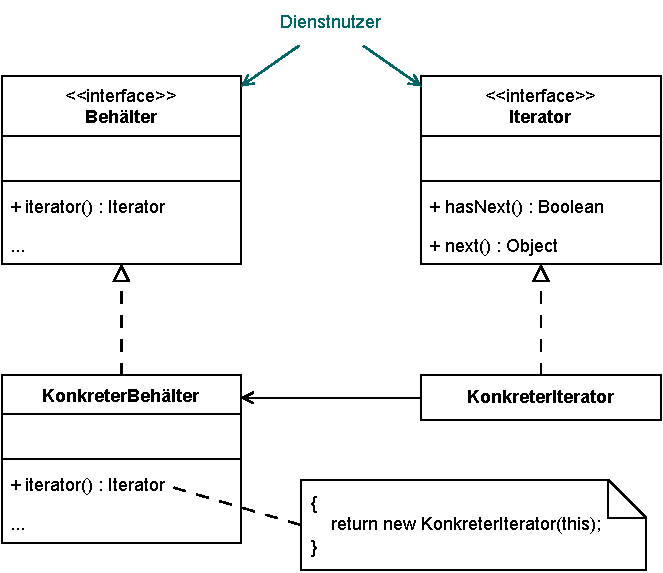
\includegraphics[scale=1.0]{Bilder/Kapitel-10/muster_iterator.pdf}
		\caption{Allgemeine Struktur des Iterator-Musters}
		\label{fig:muster_iterator}
	\end{figure}

	\item[Beteiligte] ~
	\begin{itemize}
		\item 	Das Interface Iterator definiert eine Schnittstelle mit Operationen zum sequentiellen Zugriff auf die Elemente eines Behälterobjekts.
		\item 	Die Klasse \sttpUMLText{KonkreterIterator} implementiert das Iterator-Interface und speichert den aktuellen Zustand des Behälterdurchlaufs.
		\item 	Das Interface \sttpUMLText{Behälter} definiert (neben den typischen Behälteropera\-tionen) eine Operation zum Erzeugen eines Iteratorobjekts.
		\item 	Die Klasse \sttpUMLText{KonkreterBehälter} implementiert die iterator()-Operation aus dem Behälter-Interface und liefert ein zum Behälter passendes 
		\linebreak %%% für Druck
		Iteratorobjekt.
	\end{itemize}
	
	\item[Zusammenspiel] Das konkrete Iteratorobjekt merkt sich das aktuelle Element des Behälters und kann das nächste Objekt des Durchlaufs berechnen.
	\item[Konsequenzen] Das Iterator-Muster hat folgende Vorteile:
	\begin{itemize}
		\item 	Es ermöglicht verschiedene Arten eines Behälterdurchlaufs. Beispiels\-weise kann eine Baumstruktur in verschiedenen Reihenfolgen (\zb in-order, pre-order oder post-order) durchlaufen werden. Iteratoren machen es einfach, den Durchlaufalgorithmus auszutauschen: Man tauscht einfach das Iteratorobjekt gegen ein anderes aus, das ebenfalls das Iterator-Interface implementiert.
		\item 	Iteratoren vereinfachen die Schnittstelle von Behältern, da anstelle der Durchlaufoperationen nur noch eine Operation erforderlich ist, die den Iterator erzeugt.
		\item 	Da ein Iterator den aktuellen Durchlaufzustand speichert, können mehrere Durchläufe durch einen Behälter parallel stattfinden.
	\end{itemize}	
	
\end{description}
	